\documentclass[12pt, letterpaper, twocolumn]{article}

\usepackage[utf8]{inputenc}
\usepackage[english]{babel}
\usepackage{graphicx}

\usepackage{biblatex}
\addbibresource{references.bib}

\title{Physically Based Rendering}
\author{Daichi Jameson \and Sam Sartor}
\date{May 2017}
 
\begin{document}

\begin{titlepage}
\maketitle
\end{titlepage}
 
\section{Abstract}

Physically based rendering (PBR) is a branch of computer graphics focused on
the realistic and accurate description and simulation of materials’ visual
properties. Instead of describing the appearance of an object, an artist using
PBR techniques endeavors to describe the material of the object itself. How
metallic it is, how rough, how colored. In addition to an added degree of
realism, PBR provides two additional benefits: a more intuitive method of
manipulating materials and material consistency between different lighting
environments\cite{lerpGL}. While it is physically based, realism in not a
requirement. PBR is also useful for cartoony or abstract visuals.

As a programmer, implementing physically based shading is challenging because
of the complexity and obscurity of physically accurate lighting equations.
Many are most commonly represented as massive integrals that are difficult to
convert into usable code. Our PBR implementation uses a metalness workflow
with the Cook-Torrance specular reflectance model, high dynamic range, normal
mapping, shadow mapping, and gamma correction. The resulting program is able
to create realistic and interesting images in real time.

\section{Introduction}

Developing intuitive and effective rendering techniques is a problem that has
existed since the dawn of 3D graphics. Several different lighting models have
come about in an attempt to solve this problem, with varying degrees of
success. One of the most famous lighting models is the Phong shading model,
developed around 1975 by Bui Tuong Phong\cite{panini}. While the Phong
shading model is able to create good looking scenery, it fails to account for
certain real world laws, causing certain scenes to have unrealistic
properties. More modern models account for additional real world properties,
allowing for more realistic renders to be made.
 
Physically based rendering is a broad term describing a set of rendering rules
that aims to emulate properties of the physical world in order to create
realistic environments that are intuitive to manipulate. There is no limit on
how pedantic PBR is allowed to be, but there are a few properties common to
almost all PBR implementations:  conservation of energy, the Fresnel effect,
the microfacet surface model, and differentiating between metallic and
dielectric materials\cite{PBEc}. In addition to the rules that are generally
associated with PBR, several other rendering techniques are often used to
maximize the realism of the final images.

\section{Related Work}

Physically based rendering aims to correct the consistency, realism, and
controllability issues with older techniques like Phong. The first correction
made by physically based rendering is conservation of energy. In theory, this
is a simple physics principle: the amount of energy in a system must stay
constant\cite{NERSA}. In the context of computer graphics, conservation of
energy means that the light energy leaving a surface must be less than or
equal to the light energy received by the surface (excluding emitted light)
\cite{lerpGL}. The next important concept to understand is the microfacet
surface model (Figure \ref{microfat}). Most of the optical properties
associated with real world surfaces originate with the tiny imperfections in
the surface. A model of these imperfections, when used to develop improved
shading equations, is called a microfacet model\cite{CoTor}. The Fresnel
equation, nearly ubiquitous in modern computer graphics, is an example of a
formula partially derived from microfacet models. The Fresnel equation is most
commonly used to model the increased reflectivity of materials at shallow
angles\cite{lerpGL}.

\begin{figure}
\centering 
\includegraphics[width=0.5\textwidth]{pbr_theory_microsurf.png}
\caption{Reflecting microfacets}
\label{microfat}
\end{figure}

Perhaps the biggest correction made by physically based rendering is the
distinction between metallic and non-metallic materials. To understand this
distinction, it is important to first understand the distinction between
specular (reflected) and diffuse (scattered) light. When photons hit a
surface, some reflect immediately off the surface and back into free space.
This is the specular component. The “hardness” of this reflection is due only
to the roughness of the tiny imperfections on the surface. Hence the
usefulness of microfacet models. The remainder of the photons can travel past
the first layer of atoms and into the volume of the material itself (all
materials are somewhat transparent). Here they are scattered and reflected
many times, moving in an irregular path through the object (Figure
\ref{refscat}). Many of these photons will return to the surface and travel
off in a random direction. This “scattering” creates the diffuse shading
component. Keep in mind that in both these cases, some of the photons will be
absorbed as heat before scattering or reflecting.

\begin{figure}
\centering 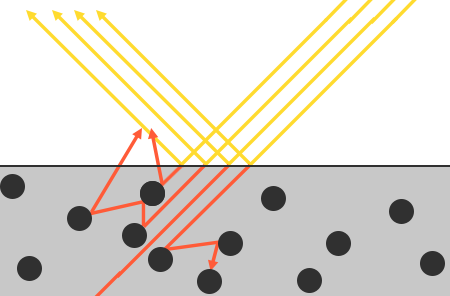
\includegraphics[width=0.5 \textwidth]{surface_reaction.png}
\caption{Reflection and scattering}
\label{refscat}
\end{figure}

Non-metallic (dielectric) materials happen to reflect all wavelengths evenly
and so have a white specular component. Color is only added during scattering.
The ratio between reflected and scattered light is described primarily by the
Fresnel equation. On the other hand, any light that passes the surface of a
metallic material will never return. Thus, metals only have a specular
component. Diffuse looking metal objects are simply rough, not truly diffuse.
Unlike dielectric objects, the ratio of reflected light is wavelength
dependent. This causes the specular component of metals to be colored
\cite{CoTor}.

There are two primary workflows used to describe the properties of a material:
the specular workflow and metalness workflow\cite{MTex}. The metalness
workflow aims to provide an intuitive method of describing materials. The
inputs to this workflow are albedo, metalness, and roughness\cite{MTex}
(Figure \ref{metalwork}). Albedo describes the color of the material. This is
the diffuse color of a dielectric and the specular color of a
metal\cite{MTex}. The metalness map then describes which of those cases
applies\cite{MTex}. The  roughness map describes the roughness of the
material, which affects the sharpness of specular reflections\cite{MTex}.
Conversely, the specular workflow aims to provide inputs similar to Phong,
where materials are described using their explicit color values\cite{MTex}.
Specular workflows use albedo, specular, and glossiness maps\cite{MTex}. An
important difference between Phong and the specular workflow is that the
specular workflow keeps all of the color information in the albedo map, and
uses the specular map to only relay information on how specular a surface
should be\cite{MTex}. Regardless of the workflow or implementation, these
inputs are almost always stored in a texture to allow for variation across an
object.

\begin{figure}
\centering 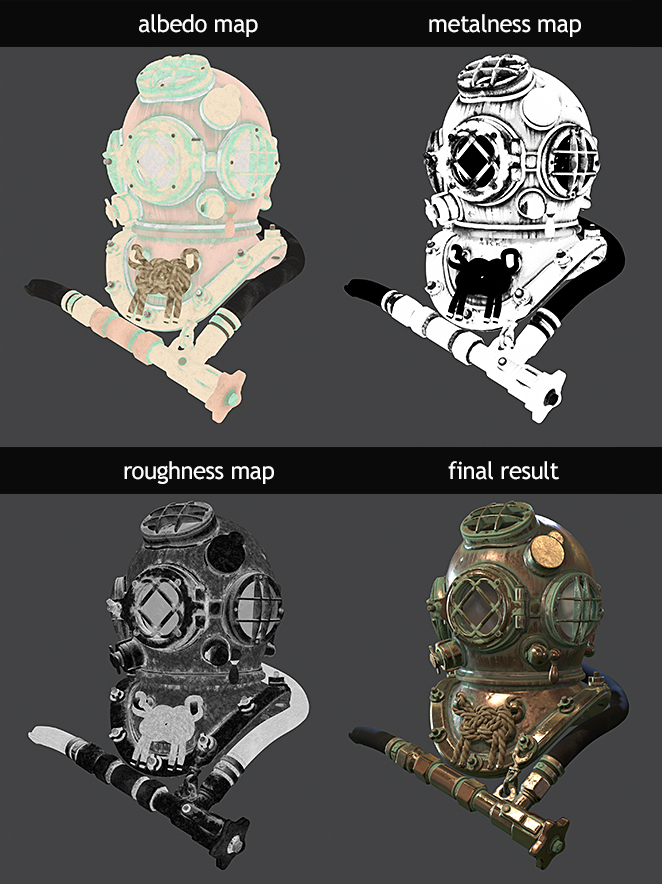
\includegraphics[height=3.2in]{metalness_workflow.jpg}
\caption{Inputs to metalness workflow}
\label{metalwork}
\end{figure}

In addition to the basic principles of physically based rendering, there are a
few other rendering techniques that allow for more realistic looking scenery.
The use of high dynamic range (HDR) and gamma correction is particularly
important to achieving realism and/or consistency. A common issue in normal
renders occurs when the final light value of a pixel exceeds 1.0. Lighting
information about the scene is then lost, and the final render becomes blown
out. High dynamic range addresses this issue by first rendering the scene on
an unbounded scale, and afterwards transforming the lighting values into the
monitor’s display range through a process called tone mapping\cite{HiDy}. Tone
mapping allows for the lighting to be scaled down into a displayable range
while still having control of the final image. Gamma correction is another
extremely important rendering technique that converts lighting values between
a linear color space and the color space monitors use to render images
\cite{GamCo}. Using gamma correction ensures that the values calculated in
shaders are physically correct, something that is critical for for physically
based rendering to be done correctly.

\section{Problem Statement}

Creating realistic renders in real time is a challenging task. While it is
currently (and may always be) impossible to simulate the world perfectly,
there are several techniques that attempt to emulate real world properties in
a computationally efficient manner whilst still preserving render quality. In
addition, it is important for materials to be easily adjustable, and for
materials to stay consistent between different lighting environments.

The Phong model is one of the most popular solutions for real time rendering.
Though it is a fairly effective solution, it has many shortcomings and does
not account for a few key physical properties, which limits the degree of
realism it can achieve. Another major disadvantage of the Phong lighting model
is the difficulty of working with material colors. The Phong lighting model
requires the user to directly manipulate the specular, diffuse, and ambient
values, which can be quite difficult to adjust in order to create realistic
looking materials. Additionally, the Phong lighting model suffers from
consistency issues on materials between different lighting environments
\cite{lerpGL}. In order to address this issue, an artist would have to go and
tweak the colors of a model to make sure that its look remains consistent
\cite{lerpGL}. Physically based rendering aims to solve these issues.

\section{Problem Solution}

We implemented this project using a language called Rust. Rust is more robust
and higher level than C++ while preserving on-the-metal performance and
access. We hoped that using Rust would make our implementation easier to code
and more robust. High-level, reliable, and multi-threadable access to OpenGL
is provided through the gfx library. In addition to OpenGL, gfx can use
DirectX 11, DirectX 12, Metal, and Vulcan as backends; however, this project
exclusively uses the OpenGL backend.

We chose to use the metalness workflow for several reasons. It seems to be
better documented, we were able to find more test models using it, and it made
more intuitive sense to us.

In addition to a basic physically based shading model, our program improves
realism using HDR rendering, gamma correction, normal mapping, and shadow
mapping.

On startup, the program loads a set of objects. Each one comprises a Wavefront
OBJ model and 4 PNG images (normal, albedo, metalness, and roughness).
Position, normal, and texture coordinates are loaded from the OBJ file and put
in vertex buffer along with calculated tangent and bitangent vectors. Triangle
indices are also loaded from the file and placed into an index buffer.
Similarly, the 4 images are loaded into opengl textures. Only the albedo
texture is in sRGB space and needs to be corrected, the others are linear
(note that this is a common convention but not universal).

The rendering step uses multi-pass techniques extensively. The first pass
renders the scene to a gbuffer, which stores position, UV, and normal
information. This step is also responsible for applying the object’s normal
map. Applying the normal map early prevents us from having to store the
tangent and bitangent in the gbuffer, reduces the number of textures being
bound by the lighting pass, and reduces the amount of work being repeated by
the lighting pass.

The next two passes are repeated per-light. First, the scene is rendered from
the light’s perspective in order to populate a shadow map. Shadow acne is
avoided by clipping front faces and only storing the depth of back faces. This
does not create any additional issues because all of our example objects are
solid.

Once the shadow pass is complete for the given light, a fullscreen quad is
rendered with the PBR fragment shader. This shader uses the Cook-Torrance
model which is energy conserving, microfacet based, and includes the Fresnel
effect\cite{CoTor}. This shader is also responsible for the shadow depth-check.
A total of 6 textures are loaded: gbuffer layer a, gbuffer layer b, the
albedo map, the metalness map, the roughness map, and the shadow map. This
shader outputs a floating-point luminance value which is added to the
luminance buffer (additive blending mode). The luminance buffer is reset every
frame, and then the contribution from each light is added to the buffer in
sequence. This allows us to include multiple shadow-casting lights into our
scene without loops or arrays in the fragment shader. By alternating between
shadow pass and lighting pass, a single shadow map is required. It can be
written over by every light because the previous light’s contribution has
already be added to the total luminance.

A final fullscreen quad is rendered to convert the 32-bit HDR luminance buffer
into an 8-bit LDR screen buffer. This final pass is responsible for gamma
correction and tone mapping.

\section{Results}

Our results are very encouraging. Using textures provided us a level of detail
and storytelling ability that would be impossible to obtain otherwise. Rust
and gfx also proved to be effective: adding new passes, buffers, shaders,
textures, etc. was clean and straightforward. The program also performed well,
handling 10 or more lights (each with shadow passes) without a noticeable
frame-rate drop. Most importantly, our objects appear consistent under
different lighting conditions. Wood looks like wood, copper looks like copper,
and steel looks like steel, regardless of what color lights we choose. If we
had the time, additional improvements could be made by adding ambient
occlusion, antialiasing, and/or image-based lighting.

\begin{figure}
\centering 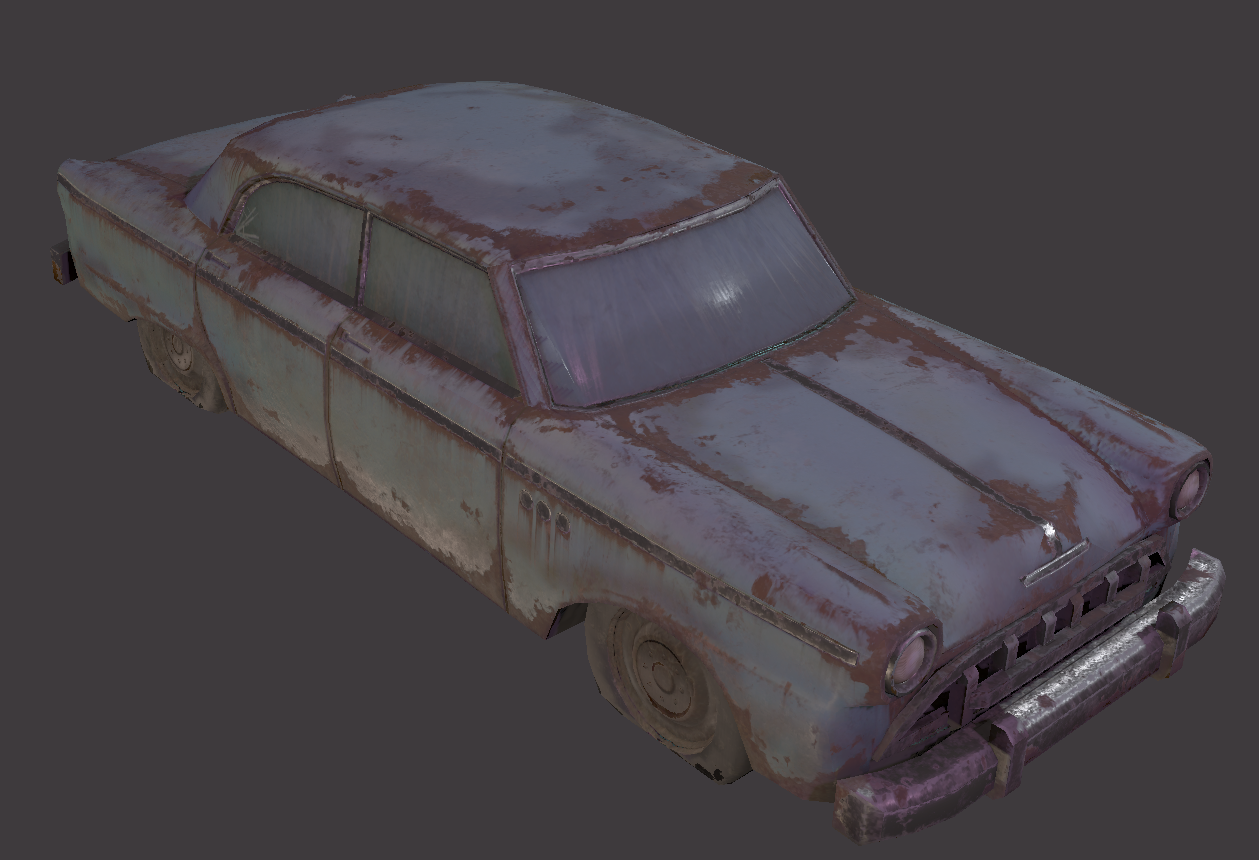
\includegraphics[width=0.5 \textwidth]{pbr_car_02.png}
\caption{Car rendered in our program}
\label{scrot}
\end{figure}

\section{Conclusion}

Throughout the history of computer graphics there have been many attempts to
model the lighting and shading of scenes. The Phong model has become one of
the most prominent and visually appealing shading model. Despite the Phong
model’s popularity, it fails to account for several properties of the real
world, such as the difference between metallic and dielectric materials, the
increase in specularity at steep angles, and the conservation of energy.
Physically based rendering is a new paradigm that appeared and declared that
the end result is not the only thing that matters, but rather that properly
modeling real world phenomena will lead to better looking, more physically
accurate results. While modeling the world as accurately as possible leads to
more complex math and more computationally intensive calculations, new
hardware has given us the ability to do these calculation in real-time.

Our implementation, while not trivial to create, does a good job demonstrating
these advantages. Through a collection of multipass techniques, we can render
a variety of complex and visually appealing objects. These advantages are
perhaps why almost all modern game engines and visual effects use physically
based rendering.

\printbibliography

\end{document}